\chapter{Eredmények}

A szoftver teszteléséhez a megtalálandó tárgy a \ref{fig:reconstr-img} ábrán látható TV-távirányító volt. A választás azért esett erre a tárgyra, mert kellően részletgazdag, és a mérete megfelelő a teszteléshez.

A tárgy pozíciójának meghatározását több elrendezésre is elvégeztem, elrendezésenként többször is lefuttatva a keresést. itt három ilyen teszt eredményét mutatom be, a tesztek során a keresést rendre 7, 7 és 6 alkalommal futtattam le. A megfogási konfiguráció ideális értékét kézzel állítottam be, ehhez képest mértem az ideális célkonfigurációt.

A három elrendezés a következő volt:

\begin{figure}[H]
\centering     %%% not \center
\subfigure[1. elrendezés]{\label{fig:arr1}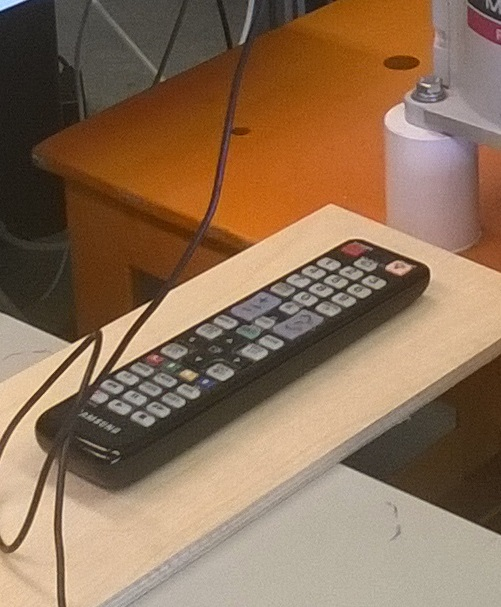
\includegraphics[height=0.56\linewidth]{chapters/results/arr1.jpg}}
\subfigure[2. elrendezés]{\label{fig:arr2}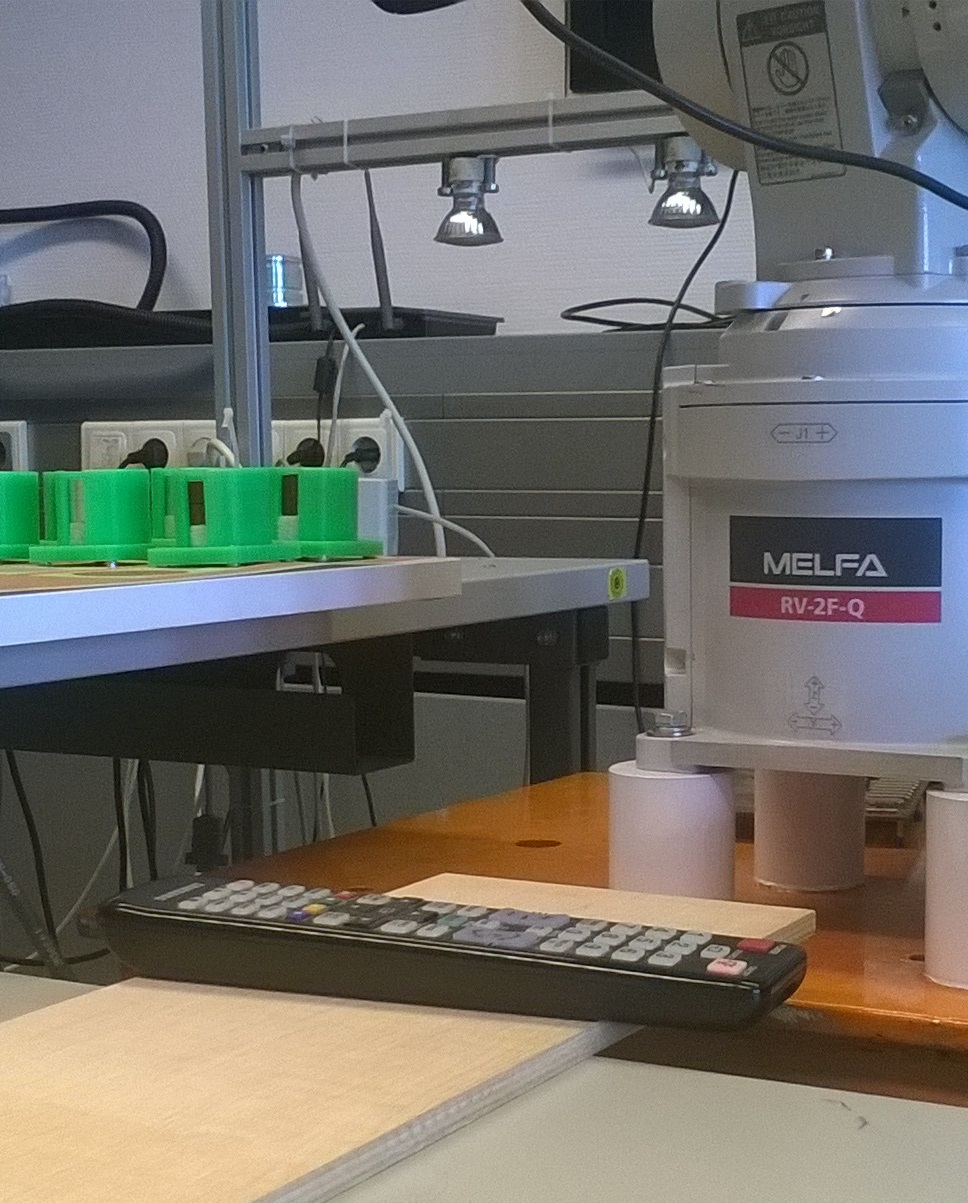
\includegraphics[height=0.56\linewidth]{chapters/results/arr2.jpg}}
\subfigure[3. elrendezés]{\label{fig:arr3}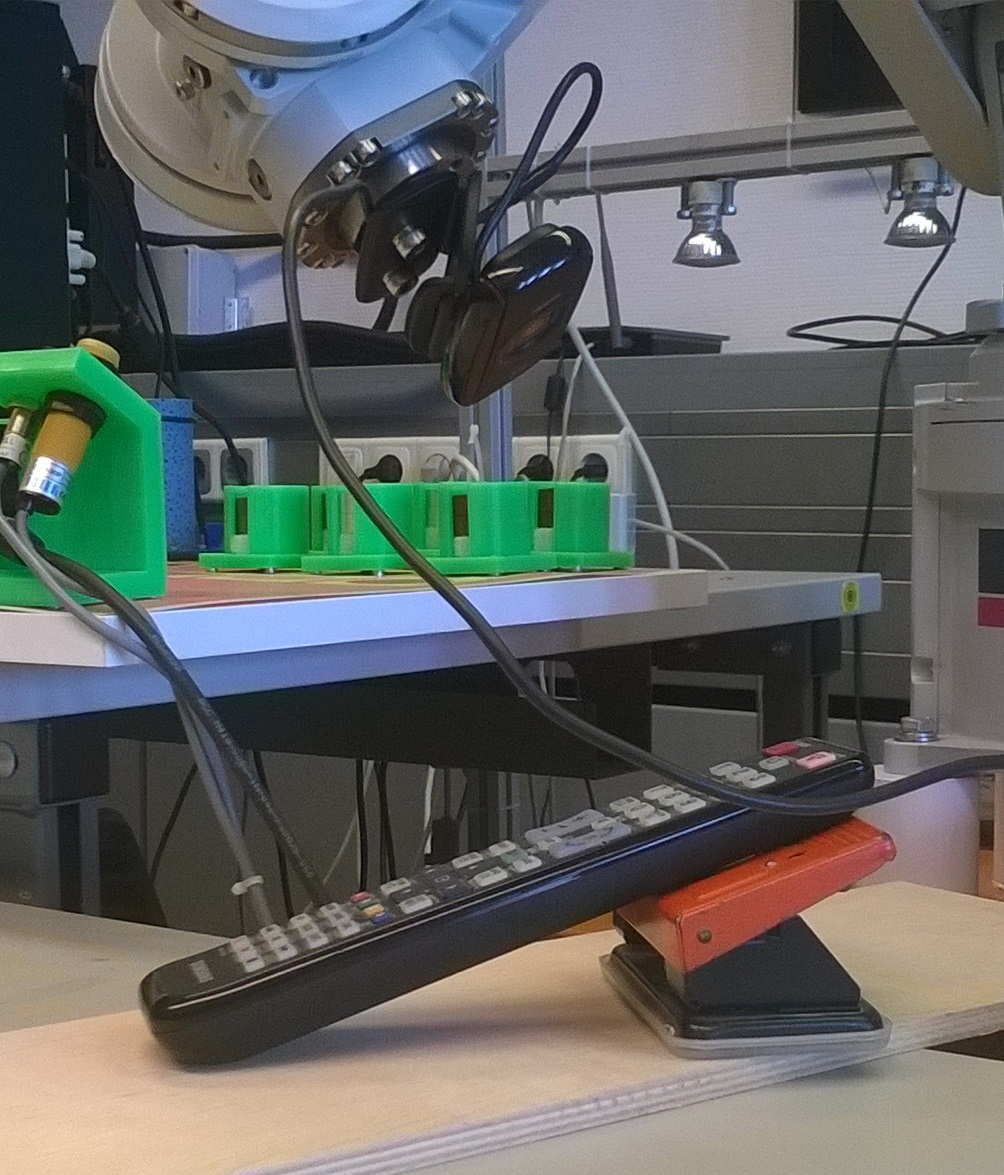
\includegraphics[width=0.45\linewidth]{chapters/results/arr3.jpg}}
\caption{A különböző elrendezések}
\end{figure}

Az eredmények közlésénél a következő jelölést használom:

\begin{itemize}
\item $\delta_x$, $\delta_y$, $\delta_z$, $\delta$ a két végpont közötti koordinátánkénti és abszolút különbség. $\delta^2=\delta_x^2+\delta_y^2+\delta_z^2$
\item $\Delta_x$, $\Delta_y$, $\Delta_z$, $\Delta$ rendre a két orientáció $x$, $y$ és $z$ tengelyei által bezárt szög és ezek számtani közepe. Amennyiben az orientációk megegyeznek, ezek természetesen nullával egyenlők.
\end{itemize}

% bevezetek egy mértéket, amely két orientáció különbözőségét méri. A helyes és a kapott orientáció eltérése úgy kerül számításra, hogy az orientációk által definiált bázisvektorok által bezárt szögek abszolút értékének vesszük az átlagát:
%
%\begin{equation}
%\Delta_{rot}(\mathbf{A}, \mathbf{B}) \coloneqq \frac{\angle (\mathbf{a}_1,\mathbf{b}_1) + \angle (\mathbf{a}_2,\mathbf{b}_2) + \angle (\mathbf{a}_3,\mathbf{b}_3)}{3} = \frac{\tr \left(\arccos\left(\mathbf{A}^T\mathbf{B}\right)\right)}{3}
%\end{equation}
%
%Ahol:
%
%\begin{equation*}
%\begin{split}
%\mathbf{A} &= \left[ \begin{array}{ccc} \mathbf{a}_1 & \mathbf{a}_2 & \mathbf{a}_3 \end{array} \right] \in \mathbb{R}^{3\times 3}, \quad \mathbf{A}^{-1} = \mathbf{A}^T \\
%\mathbf{B} &= \left[ \begin{array}{ccc} \mathbf{b}_1 & \mathbf{b}_2 & \mathbf{b}_3 \end{array} \right] \in \mathbb{R}^{3\times 3}, \quad \mathbf{B}^{-1} = \mathbf{B}^T
%\end{split}
%\end{equation*}
%
%A definícióból szemléletesen adódnak a következő tulajdonságok:
%
%\begin{itemize}
%\item $\Delta_{rot}(\mathbf{A}, \mathbf{A}) = 0$
%\item $\Delta_{rot}(\mathbf{A}, \mathbf{-A}) = \pi$
%\item $0 \leq \Delta_{rot}(\mathbf{A}, \mathbf{B}) \leq \pi$
%\end{itemize}

Az eredményeket a következő táblázatok mutatják.

%x, y, z trans eltérések, trans eltérés (gyök(négyzetösszeg)), x, y, z tengely szögeltérés, rot eltérés, inlierek sz. (trans cm-ben, rot fokban)
%data1
%[ 4.23  1.07  2.1 ], 4.84, [ 32.24  21.74  28.28], 27.42, 189
%[ 0.46 -1.5   4.63], 4.89, [ 21.62  21.62   0.4 ], 14.55, 157
%[ 0.81  0.02  4.08], 4.16, [ 6.6   5.96  2.99], 5.18, 76
%[ 4.32  1.06  1.97], 4.86, [ 32.58  22.76  27.9 ], 27.75, 183
%[-0.15 -0.64 -1.61], 1.74, [ 44.05  16.33  41.91], 34.10, 130
%[-0.38 -0.3  -1.91], 1.97, [ 32.07   3.97  31.89], 22.65, 152
%[ 0.33  0.07  2.25], 2.27, [ 10.13   0.37  10.14], 6.88, 101
%data2
%[ 1.76 -0.58 -5.35], 5.66, [ 46.07  72.06  73.97], 64.04, 116
%[ 0.16 -2.24  4.23], 4.79, [ 77.6   60.79  81.67], 73.35, 251
%[ 4.24  0.31  3.56], 5.55, [ 61.48  96.44  81.65], 79.86, 187
%[ 0.   -2.25  4.16], 4.73, [ 78.7   60.98  81.6 ], 73.76, 274
%[ 0.14 -0.75  3.92], 3.99, [ 71.36  86.41  81.74], 79.84, 248
%[ 0.03 -2.61  3.29], 4.20, [ 76.88  65.43  81.36], 74.56, 212
%[-0.11 -0.72  3.72], 3.79, [ 66.29  84.23  81.89], 77.47, 209
%data3
%[ 4.64  3.   -6.46], 8.50, [ 14.34  34.55  32.73], 27.21, 61
%[ 1.59 -0.34  3.19], 3.58, [ 14.79  29.02  28.64], 24.15, 115
%[ 1.93 -0.63 -3.54], 4.08, [ 27.74  21.12  35.02], 27.96, 71
%[ 4.28 -0.52 -5.48], 6.97, [ 53.73  51.96  36.13], 47.27, 29
%[ 1.31 -1.03  5.48], 5.73, [ 17.85  30.25  25.74], 24.61, 100
%[ 1.17 -0.65  4.08], 4.30, [ 15.56  27.4   22.42], 21.79, 190
%
%data1\\
%4.23&	1.07&	2.1&	4.84&	32.24&	21.74&	28.28&	27.42&	189\\
%0.46&	-1.5&	4.63&	4.89&	21.62&	21.62&	0.4&	14.55&	157\\
%0.81&	0.02&	4.08&	4.16&	6.6&	5.96&	2.99&	5.18&	76\\
%4.32&	1.06&	1.97&	4.86&	32.58&	22.76&	27.9&	27.75&	183\\
%-0.15&	-0.64&	-1.61&	1.74&	44.05&	16.33&	41.91&	34.10&	130\\
%-0.38&	-0.3&	-1.91&	1.97&	32.07&	3.97&	31.89&	22.65&	152\\
%0.33&	0.07&	2.25&	2.27&	10.13&	0.37&	10.14&	6.88&	101\\
%data2\\
%1.76&	-0.58&	-5.35&	5.66&	46.07&	72.06&	73.97&	64.04&	116\\
%0.16&	-2.24&	4.23&	4.79&	77.6&	60.79&	81.67&	73.35&	251\\
%4.24&	0.31&	3.56&	5.55&	61.48&	96.44&	81.65&	79.86&	187\\
%0.&	-2.25&	4.16&	4.73&	78.7&	60.98&	81.6&	73.76&	274\\
%0.14&	-0.75&	3.92&	3.99&	71.36&	86.41&	81.74&	79.84&	248\\
%0.03&	-2.61&	3.29&	4.20&	76.88&	65.43&	81.36&	74.56&	212\\
%-0.11&	-0.72&	3.72&	3.79&	66.29&	84.23&	81.89&	77.47&	209\\
%data3\\
%4.64&	3.&	-6.46&	8.50&	14.34&	34.55&	32.73&	27.21&	61\\
%1.59&	-0.34&	3.19&	3.58&	14.79&	29.02&	28.64&	24.15&	115\\
%1.93&	-0.63&	-3.54&	4.08&	27.74&	21.12&	35.02&	27.96&	71\\
%4.28&	-0.52&	-5.48&	6.97&	53.73&	51.96&	36.13&	47.27&	29\\
%1.31&	-1.03&	5.48&	5.73&	17.85&	30.25&	25.74&	24.61&	100\\
%1.17&	-0.65&	4.08&	4.30&	15.56&	27.4&	22.42&	21.79&	190\\

\setlength\tabcolsep{6pt}
\begin{table}[H]
\centering
\begin{tabular}{|rrr|r|rrr|r|c|}
\hline 
$\delta_x$ (cm) & $\delta_y$ (cm) & $\delta_z$ (cm) & $\delta$ (cm) & $\Delta_x$ (°) & $\Delta_y$ (°) & $\Delta_z$ (°) & $\Delta$ (°) & inlierek száma \\ \hline
 4.23&	1.07&	2.1&	4.84&	28.28&	21.74&	32.24&	27.42&	189\\
 0.46&	-1.5&	4.63&	4.89&	0.4&	21.62&	21.62&	14.55&	157\\
 0.81&	0.02&	4.08&	4.16&	2.99&	5.96&	6.6&	5.18&	76\\
 4.32&	1.06&	1.97&	4.86&	27.9&	22.76&	32.58&	27.75&	183\\
 -0.15&	-0.64&	-1.61&	1.74&	41.91&	16.33&	44.05&	34.10&	130\\
 -0.38&	-0.3&	-1.91&	1.97&	31.89&	3.97&	32.07&	22.65&	152\\
 0.33&	0.07&	2.25&	2.27&	10.14&	0.37&	10.13&	6.88&	101\\
\hline
\end{tabular}
\caption{Az 1. elrendezés eredményei}
\end{table}

\begin{table}[H]
\centering
\begin{tabular}{|rrr|r|rrr|r|c|}
\hline 
$\delta_x$ (cm) & $\delta_y$ (cm) & $\delta_z$ (cm) & $\delta$ (cm) & $\Delta_x$ (°) & $\Delta_y$ (°) & $\Delta_z$ (°) & $\Delta$ (°) & inlierek száma \\ \hline
 1.76&	-0.58&	-5.35&	5.66&	11.25&	34.15&	35.77&	27.06&	116\\
 0.16&	-2.24&	4.23&	4.79&	27.93&	4.36&	28.2&	20.16&	251\\
 4.24&	0.31&	3.56&	5.55&	12.45&	19.&	22.76&	18.07&	187\\
 0.&	-2.25&	4.16&	4.73&	27.8&	3.06&	27.92&	19.59&	274\\
 0.14&	-0.75&	3.92&	3.99&	2.02&	8.85&	8.71&	6.52&	248\\
 0.03&	-2.61&	3.29&	4.20&	23.13&	4.56&	23.5&	17.06&	212\\
 -0.11&	-0.72&	3.72&	3.79&	3.34&	13.95&	14.01&	10.44&	209\\
\hline
\end{tabular}
\caption{A 2. elrendezés eredményei}
\end{table}

\begin{table}[H]
\centering
\begin{tabular}{|rrr|r|rrr|r|c|}
\hline 
$\delta_x$ (cm) & $\delta_y$ (cm) & $\delta_z$ (cm) & $\delta$ (cm) & $\Delta_x$ (°) & $\Delta_y$ (°) & $\Delta_z$ (°) & $\Delta$ (°) & inlierek száma \\ \hline
 4.64&	3.&	-6.46&	8.50&	5.87&	39.6&	39.71&	28.39&	61\\
 1.59&	-0.34&	3.19&	3.58&	13.12&	16.53&	20.95&	16.87&	115\\
 1.93&	-0.63&	-3.54&	4.08&	26.85&	32.2&	39.79&	32.94&	71\\
 4.28&	-0.52&	-5.48&	6.97&	18.82&	75.&	75.08&	56.30&	29\\
 1.31&	-1.03&	5.48&	5.73&	10.83&	10.03&	14.32&	11.73&	100\\
 1.17&	-0.65&	4.08&	4.30&	4.02&	9.03&	9.64&	7.56&	190\\
\hline
\end{tabular}
\caption{A 3. elrendezés eredményei}
\end{table}

Az alábbi diagramok azt szemléltetik, hogy a különböző mennyiségű inliernél az egyes hibák mekkorák. A keresésnél a program végül 5 mérés eredményéből veszi a legjobbat (legtöbb inlier alapján számítottat). Ezeken az ábrákon mindegyik mérés szerepel, nem csak a legjobbak, mint a fenti táblázatokban.

\begin{figure}[H]
\centering
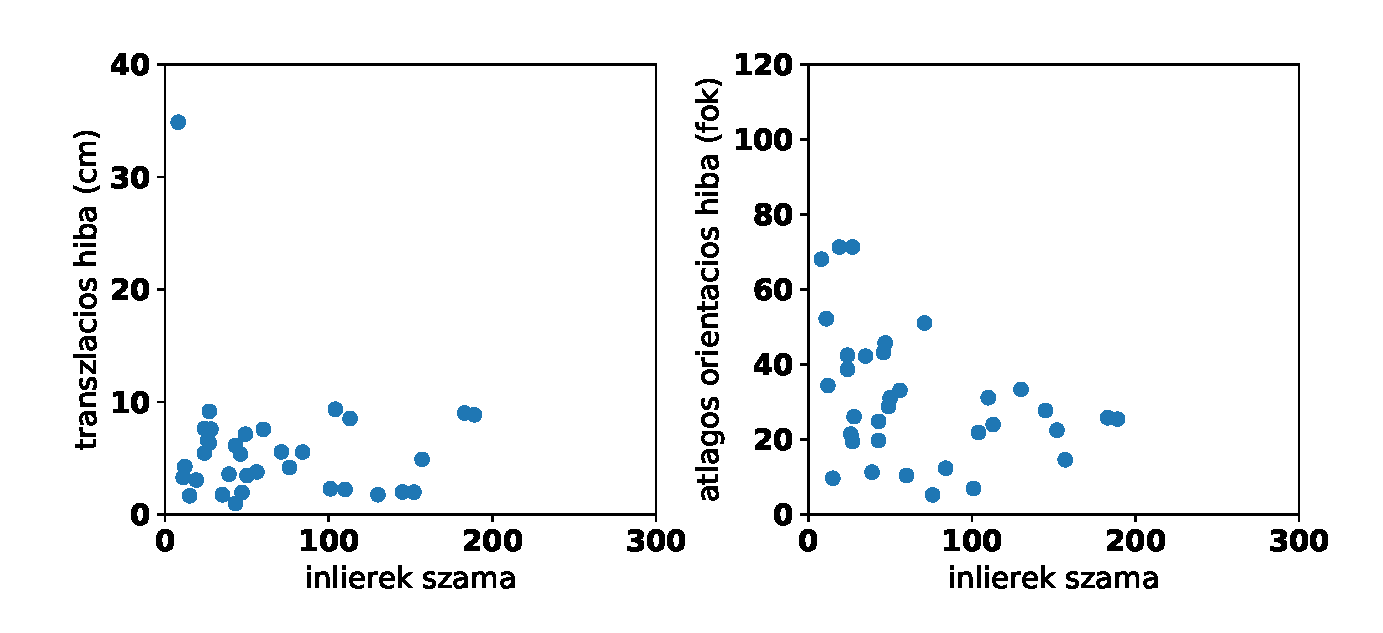
\includegraphics[width=0.9\linewidth]{chapters/results/err1.eps}
\caption{A teszt eredménye az 1. elrendezés esetében.}
\label{fig:scatter1}
\end{figure}

\begin{figure}[H]
\centering
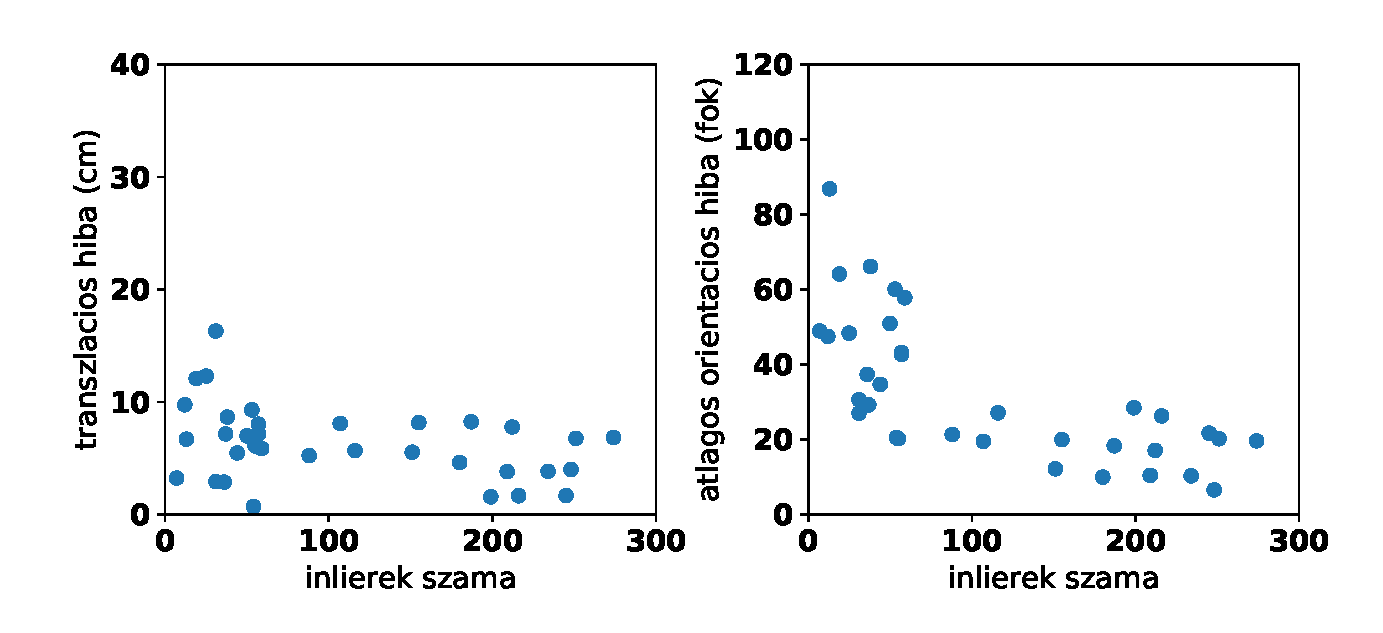
\includegraphics[width=0.9\linewidth]{chapters/results/err2.eps}
\caption{A teszt eredménye a 2. elrendezés esetében.}
\label{fig:scatter2}
\end{figure}

\begin{figure}[H]
\centering
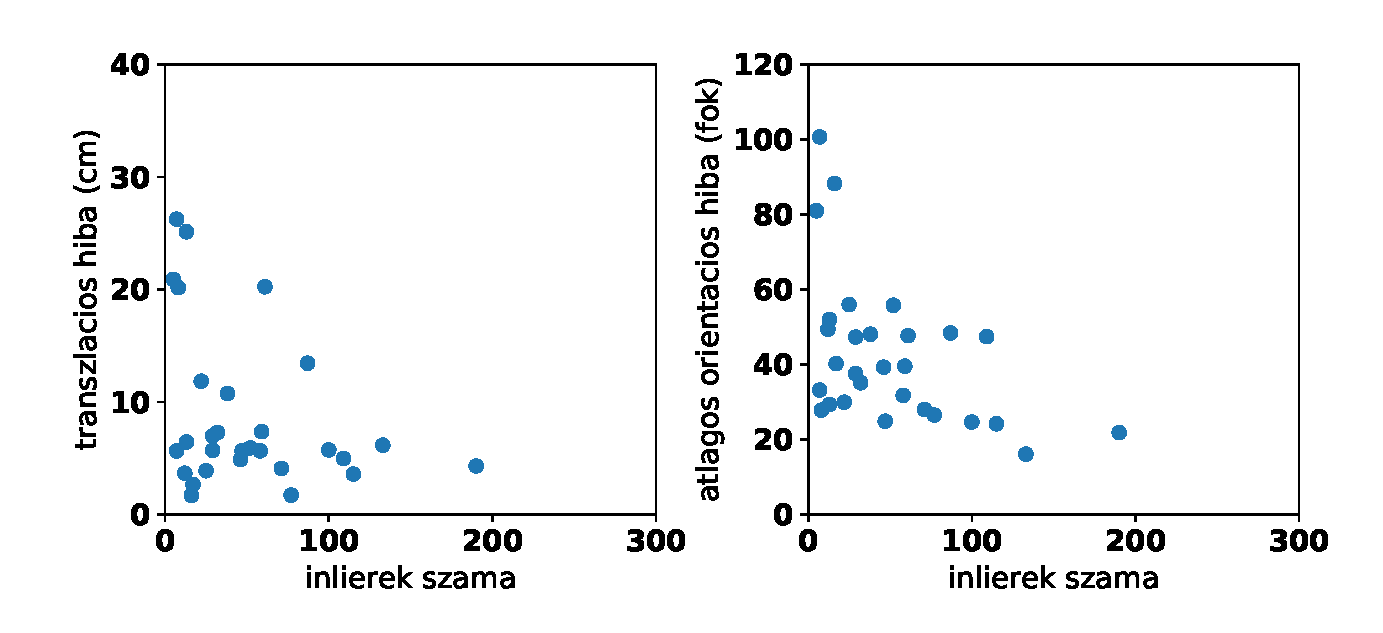
\includegraphics[width=0.9\linewidth]{chapters/results/err3.eps}
\caption{A teszt eredménye a 3. elrendezés esetében.}
\label{fig:scatter3}
\end{figure}